\subsection{\textcolor{Turquoise}{Auswertung der Effizienz (H$_{2}$)}}
\label{ch:Ergebnisse:sec:Hypothesen_Auswertung:sub:Effizienz}
% Usability = 
% - Efficiency: How quickly and with how much effort can users achieve their goals? This includes factors like time taken, number of steps, and cognitive load.
% Einfluss von Erlernbarkeit, Selbstbeschreibungsfähigkeit, Aufgabenangemessenheit
Ein System ist effizient, wenn ein Nutzer dieses schnell und ohne großen Aufwand bedienen kann. Die Bewertung umfasst die nötige Zeit, die Anzahl der Schritte und die benötigte kognitive Belastung zum Erreichen eines Ziels (s. \autoref{ch:SdF:UI:ISO})

\noindent
Folgende Hypothese ist zu bestätigen:
\begin{quote}
    H$_{2}$ = Die Nutzung des neuen Systems ($\mu2$) beeinflusst die Effizienz ($e$) der gestellten Aufgaben positiv im Vergleich zur Nutzung des alten Systems ($\mu1$); \textcolor{red}{TODO: $e(\mu1) > e(\mu2)$}.
\end{quote}

\textcolor{red}{TODO: Übergang von Hypothese zu Text smoothen.}\\
Während der Bearbeitung der Aufgaben des Usability-Tests wurde die verwendete Zeit bis zur Beantwortung aufgezeichnet. Deren Mittelwerte sind vergleichend in \autoref{fig:usability_test:zeit} dargestellt. Es ist erkennbar, dass die Bearbeitung der Aufgaben mit dem Dashboard schneller erfolgte. Die Nutzer benötigten rund 64\% der Zeit die sie mit dem alten System benötigten.

\begin{figure}[H]
    \centering
    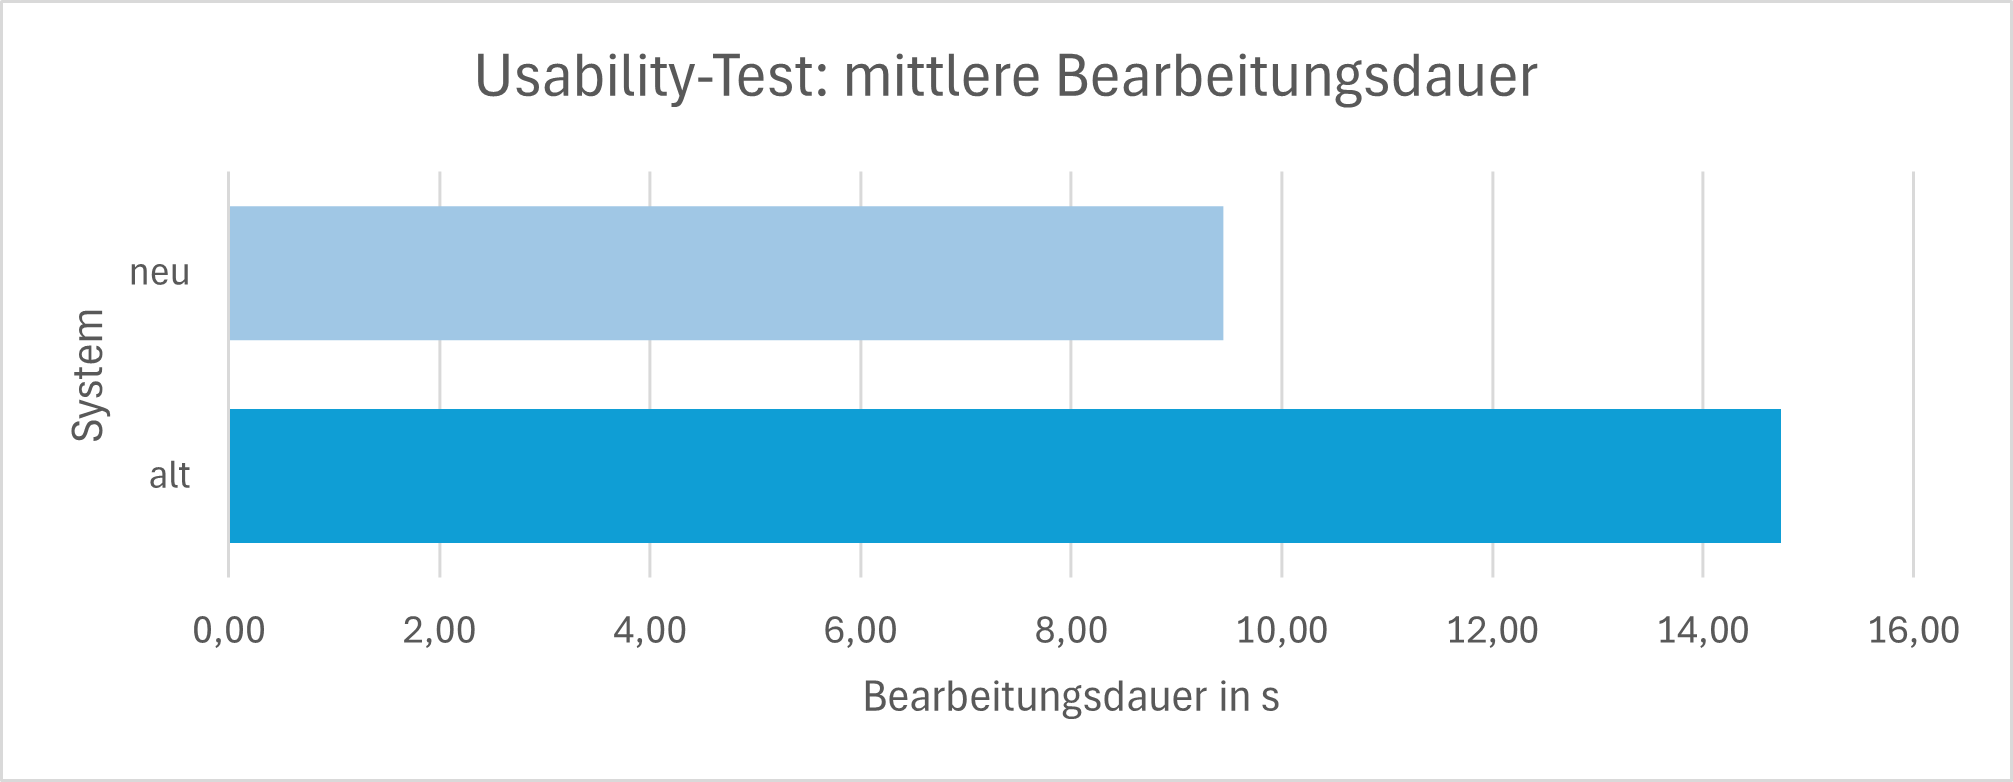
\includegraphics[width=1\linewidth]{Diagramme/usability_mittlere_zeit_2.png}
    \caption{Usability-Test: Vergleich der mittleren Bearbeitungsdauer (Weiterverarbeitung der Daten aus \autoref{tab:usability_test:mittelwerte}) \textcolor{red}{ - TODO: alt/neu tauschen}}
    \label{fig:usability_test:zeit}
\end{figure}

-> signifikant: 0,0001747 \textcolor{red}{TODO: \autoref{TODO}}

Fehlerquote s. \autoref{fig:usability_test:fehlerquote}


% ****************************************************************************************
\begin{figure}[H]
    \centering
    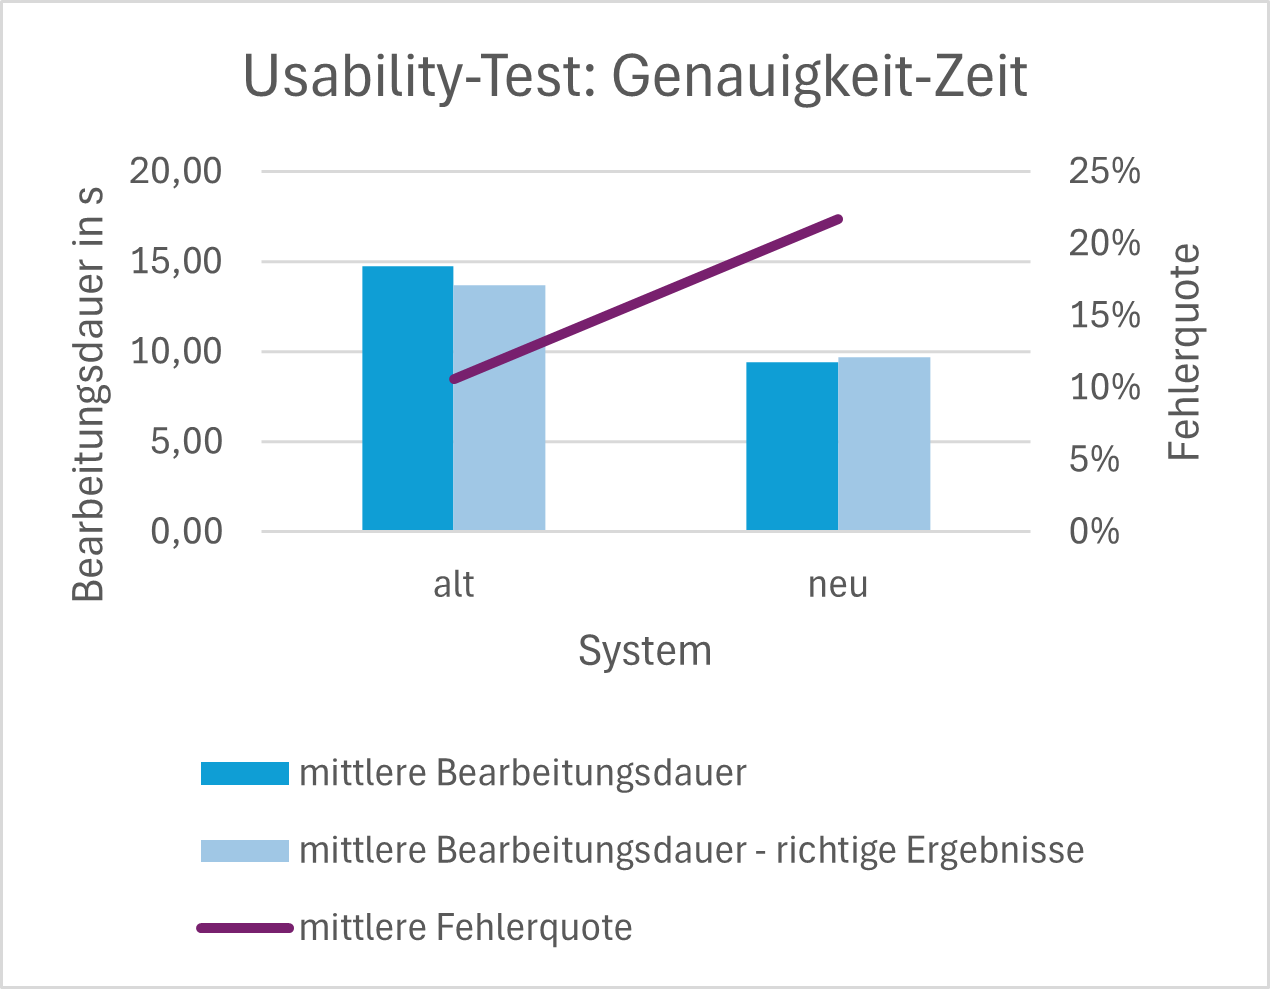
\includegraphics[width=0.8\linewidth]{Diagramme/usability_genauigkeit-zeit_mittel.png}
    \caption{Usability-Test: Vergleich der mittleren Bearbeitungsdauer - im Verhältnis zur Fehlerquote (Daten aus \autoref{fig:usability_test:fehlerquote} und \autoref{fig:usability_test:zeit}) \textcolor{red}{- TODO: Legende anpassen: 'fehlerfrei' statt 'richtig'}}
    \label{fig:usability_test:genauigkeit-zeit_mittel}
\end{figure}

\noindent
=> \autoref{fig:usability_test:genauigkeit-zeit_mittel}\\
- neu ist im Mittel schneller\\
- aber auch Fehlerquote bei neu im Mittel höher\\
%- schöne Zusammenfassung (man kann auch darauf vorspringen)

% ************************************************************
\begin{table}[H]
\begin{tabular}{ll}
$f_{alt} = \dfrac{n_{\text{\textit{gültige}}} - n_{richtige}}{n_{\text{\textit{gültige}}}}$ & // Fehlerquote \\
$e_{alt} = \dfrac{\overline{t_{alt}} } { 1 - f_{alt} }$                   & // Effizienz$_{alt}$ \\
%$e_{neu} = \dfrac{\overline{t_{neu}} } { 1 - f_{neu} }$                   & // Effizienz$_{neu}$ \\
$e_{neu:alt} = -1 * (1 - \dfrac{e_{alt}} {e_{neu}})$                      & // Verhältnis: Effizienz$_{neu}$ zu Effizienz$_{alt}$
\end{tabular}
\end{table}

\noindent
- mit dieser Formel wurden die Werte aus \autoref{fig:usability_effizienz} berechnet\\
-> Verhältnis $e_{neu}:e_{alt}$\\
$\implies$ Aufgabe 1: neues System ist zu 53,25\% effizienter als das alte System\\
$\implies$ Aufgabe 3.1: neues System ist zu 11,95\% ineffizienter als das alte System\\
$\implies$ $\varnothing$: neues System ist zu 48,46\% effizienter als das alte System\\

\begin{figure}[H]
    \centering
    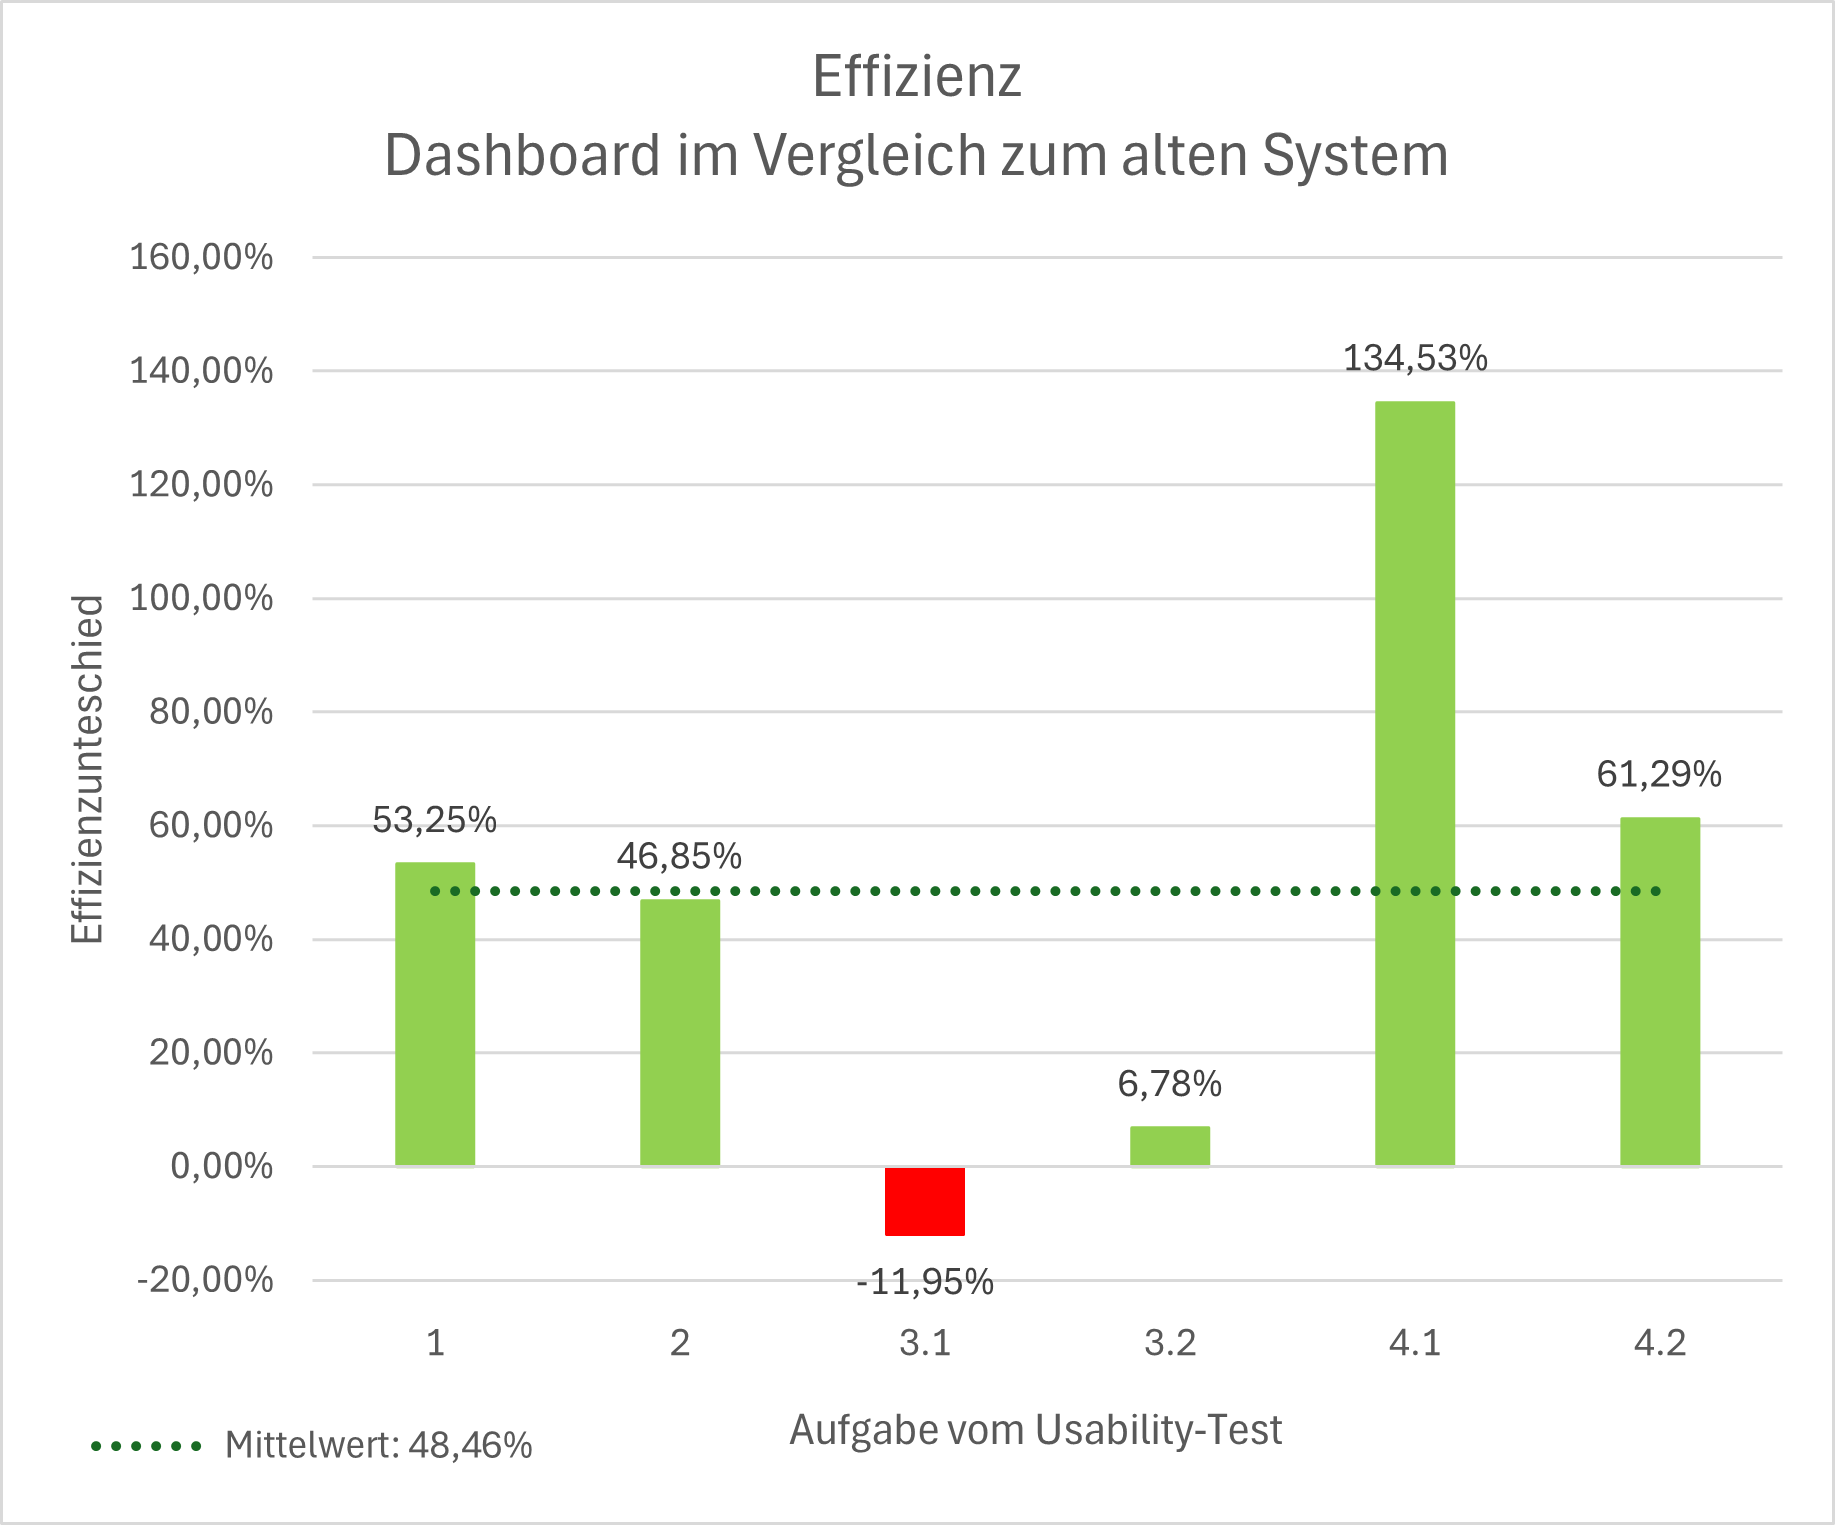
\includegraphics[width=0.8\linewidth]{Diagramme/usability_effizienz.png}
    \caption{Usability-Test: Effizienzvergleich vom neuen mit dem alten System\newline
    (Weiterverarbeitung der Daten aus \autoref{fig:usability_test:genauigkeit-zeit_alt-neu})}
    \label{fig:usability_effizienz}
\end{figure}

% ************************************************************
\noindent
\textcolor{red}{TODO: ISO-Grafiken}
%\subsection*{ISO-Kriterium Erlernbarkeit}
\begin{figure}[H]
    \centering
    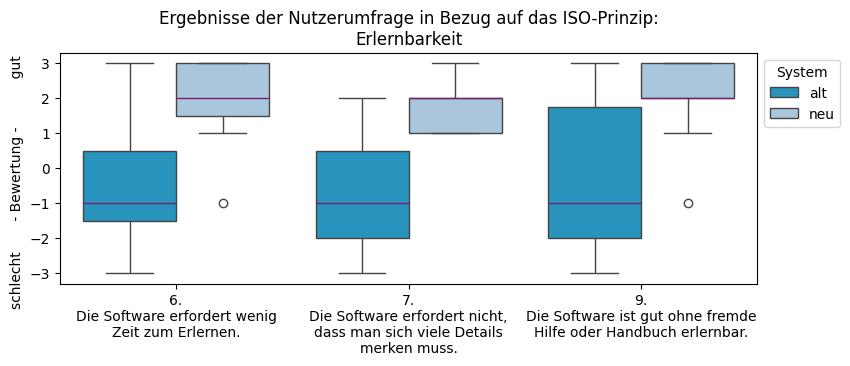
\includegraphics[width=1\linewidth]{Diagramme/pruemper_if.png}
    \caption{Auswertung der Fragen bzgl. Gestaltungskriterium Erlernbarkeit nach ISO 9241-110 (Ausschnitt aus \autoref{fig:pruemper_all})}
    \label{fig:pruemper_Erlernbarkeit}
\end{figure}

\noindent
t-Test von Fragen 6, 7 \& 9 sind signifikant (<0.5) - s. \autoref{tab:Nutzerbefragung:Differenz+ttest}\\
Boxplot: \autoref{fig:pruemper_Erlernbarkeit}
%\subsection{ISO-Kriterium Selbstbeschreibungsfähigkeit}
\begin{figure}[H]
    \centering
    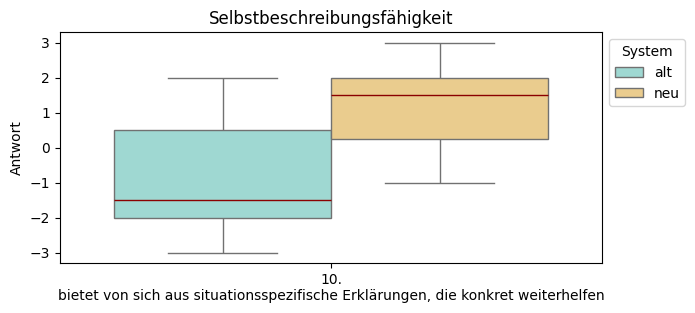
\includegraphics[width=1\linewidth]{Diagramme/pruemper_sb.png}
    \caption{Auswertung der Fragen bzgl. Gestaltungskriterium Selbstbeschreibungsfähigkeit nach ISO 9241-110 (Ausschnitt aus \autoref{fig:pruemper_all})}
    \label{fig:pruemper_Selbstbeschreibungsfähigkeit}
\end{figure}

\noindent
t-Test von Fragen 1 \& 8 sind signifikant (<0.5)\\
Boxplot: \autoref{fig:pruemper_Selbstbeschreibungsfähigkeit}

%\subsection*{ISO-Kriterium Aufgabenangemessenheit}
%\autoref{fig:pruemper_Aufgabenangemessenheit}
%\subsection*{weitere: Steuerbarkeit, Erwartungskonformität, Robustheit gegen Benutzungsfehler}
